\documentclass[11pt,a4paper]{article}
\usepackage{graphicx}
\usepackage{caption}
\usepackage{subcaption}
\usepackage[utf8]{inputenc}
\usepackage{amsmath}
\usepackage{amsfonts}
\usepackage{easy-todo}
\usepackage{amssymb}
\usepackage[left=3cm,right=3cm,top=3cm,bottom=4cm]{geometry}
\usepackage[colorlinks,linkcolor=black,citecolor=black,filecolor=black]{hyperref}
\usepackage{listings}
\catcode`^=\active
\def^#1^{\texttt{#1}}

\begin{document}
\title{Autonomous Agents - Assignment 1}
\author{Bas Veeling (10767770) \and Sebastian Droeppelmann (5783453) \and Fritjof Buettner (10876782)}
\maketitle
%\listoftodos
\section{Introduction}
\subsection{Project structure}
We decided to model the predator/prey problem in Python. We chose an object-oriented structure to make the code reusable and minimize repetitions. In order to assure correct functionality of the algorithms at a fine-grained level, we make use of Python's unit-test framework.
\begin{figure}[h!]
  \centering
    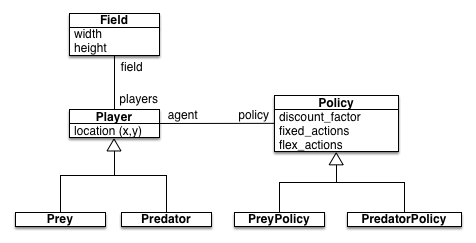
\includegraphics[width=0.6\textwidth]{classdiagram}
  \caption{Simulator Class diagram}
   \label{fig:classdiagram}
\end{figure}

The file \texttt{main.py} in the root directory of the project executes all the tasks required in the assignment and prints the according output to the console. The models for field, players and their respective policies are located in the subdirectory \texttt{models}. Their relationship is illustrated in figure~\ref{fig:classdiagram}. Both \texttt{Predator} and \texttt{Prey} class are children of the \texttt{Player} superclass, which provides common attributes such as the location and policy fields. 

There is a bidirectional connection between the field and the players on it, such that the field maintains a list of active players, who in return hold a reference to the field they are on in order to receive sensory information like the position of other players. The predator is governed by a PredatorPolicy. The prey is governed by a RandomPreyPolicy, but is not considered an agent.
Furthermore, the field also provides the function \texttt{is\_ended()} which can be used to check whether the predator has caught the prey.

For a more human-readable output, the field implements the function \texttt{print\_field()} which prints an ASCII-graphical representation of the field to the console, with a \textbf{\texttt{X}} denoting the position of the predator(s) and a \textbf{\texttt{O}} denoting the position of the prey(s).

\section{Question 1: Environment Simulator}
We implemented the simulator as described above. The ^random\_policy.py^ ^run\_random\_policy()^ function runs one simulation with a random policy for both the prey and the predator. It initializes a 11x11 field with one predator and one prey. For every time step the predator performance an action based on its policy (^predator.act()^), and this will update the field, until the game is over (^field.is\_ended()^).

The ^random\_policy\_wrapper^ function calls this simulation 100 times and calculates the average and stdev of the running time, this results in:
\begin{lstlisting}[language=bash]
Mean runtime: 0.04178s (standard deviation: 0.01846)
Mean number of iterations: 281.74 (standard deviation: 220.677)
\end{lstlisting}

\subsection{Random Policy}
The random policy of the predator is implemented in ^random\_predator\_policy.py^. The function ^get\_probability\_mapping(state)^ returns a mapping of probabilities to actions, and the super class ^Policy^ uses this to pick a next action in the function \\^pick\_next\_action(state, style)^.



\section{Question 2: Iterative policy evaluation}
Iterative Policy Evaluation is implemented in ^iterative\_policy\_evaluation.py^. It follows the algorithm described in section 4.1 of Sutton \& Barto.
We get the following results:\\
^Number of Iterations:  14\\
Predator(0,0), Prey(5,5):  0.00592929646611\\
Predator(2,3), Prey(5,4):  0.21710271406\\
Predator(2,10), Prey(10,0):  0.217283726157\\
Predator(10,10), Prey(0,0):  1.48016672878^

\section{Question 3: Policy Iteration}
Policy Iteration is implemented in ^policy\_iteration.py^. It follows the algorithm described in section 4.3 of Sutton \& Barto.
We get the following results:\\
^Gamma = 0.1 took 15 iterations and 230.68 seconds to converge.\\
Gamma = 0.5 took 12 iterations and 232.26 seconds to converge.\\
Gamma = 0.7 took 8 iterations and 220.06 seconds to converge.\\
Gamma = 0.9 took 2 iterations and 370.08 seconds to converge.\\^

\section{Question 4: Value Iteration}
Value Iteration is implemented in ^value\_iteration.py^. The main part of the value iteration algorithm is implemented in the ^while go\_on:^ loop. The code is a translation of the algorithm explained in figure 4.5 of the book. Value calculation is done in  ^calculate\_value(\dots)^. This function is slightly cumbersome due to implementation choices made earlier, but properly calculates the value as prescribed in the algorithm. A heatmap of the values can be found in figure~\ref{fig:1}.

We compute the values for discount factors of $0.1, 0.5, 0.7$ and $0.9$. This results in the following output:
\begin{lstlisting}[language=bash]
Gamma = 0.1 took 6 iterations and 28.052 seconds to converge.
Gamma = 0.5 took 7 iterations and 32.23 seconds to converge.
Gamma = 0.7 took 7 iterations and 32.04 seconds to converge.
Gamma = 0.9 took 7 iterations and 31.81 seconds to converge.
\end{lstlisting}

\begin{figure}[h!] 
  \centering
  \begin{subfigure}[t]{.45\textwidth}
    \centering
    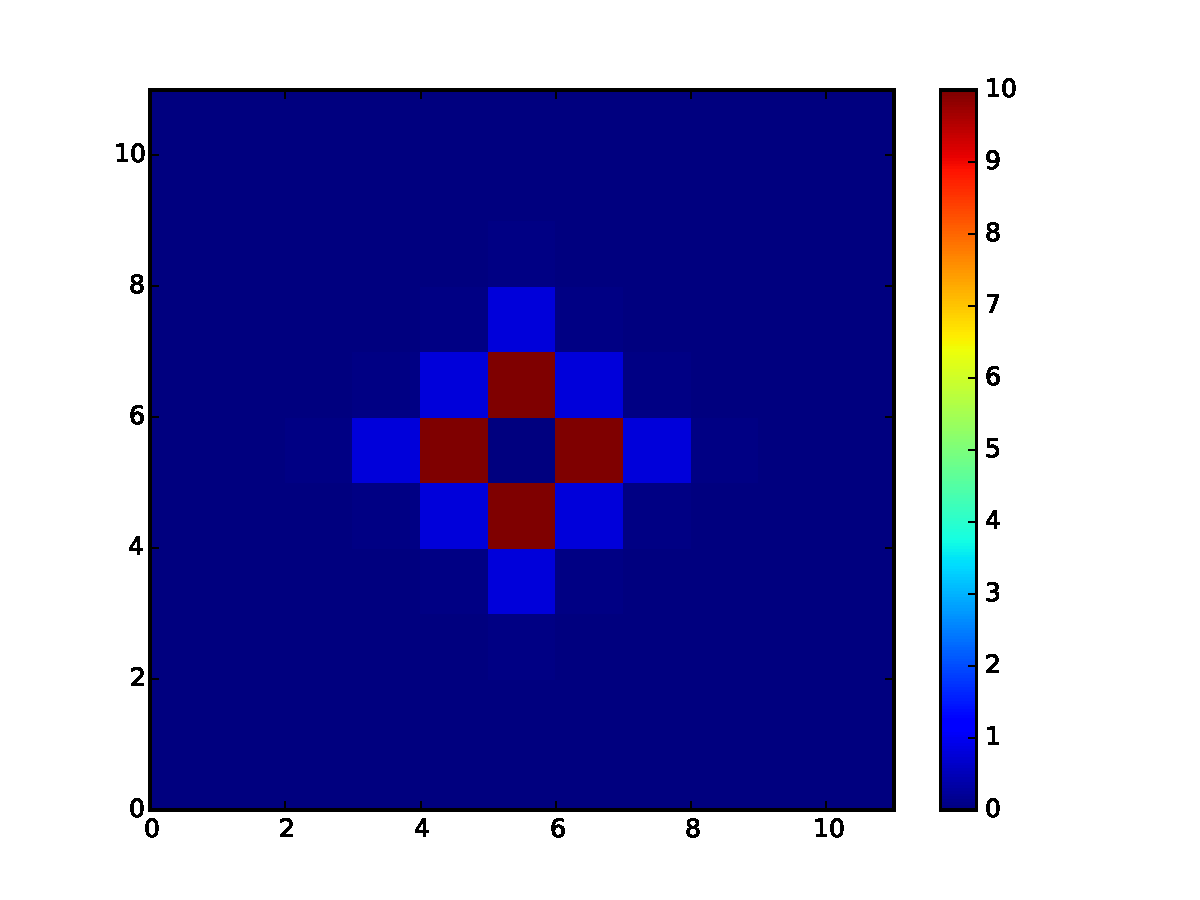
\includegraphics[width=\textwidth]{valueiteration_gamma0-1}
    \caption{$\gamma$ = 0.1}\label{fig:1a}   
  \end{subfigure}
  \quad
  \begin{subfigure}[t]{.45\textwidth}
    \centering
    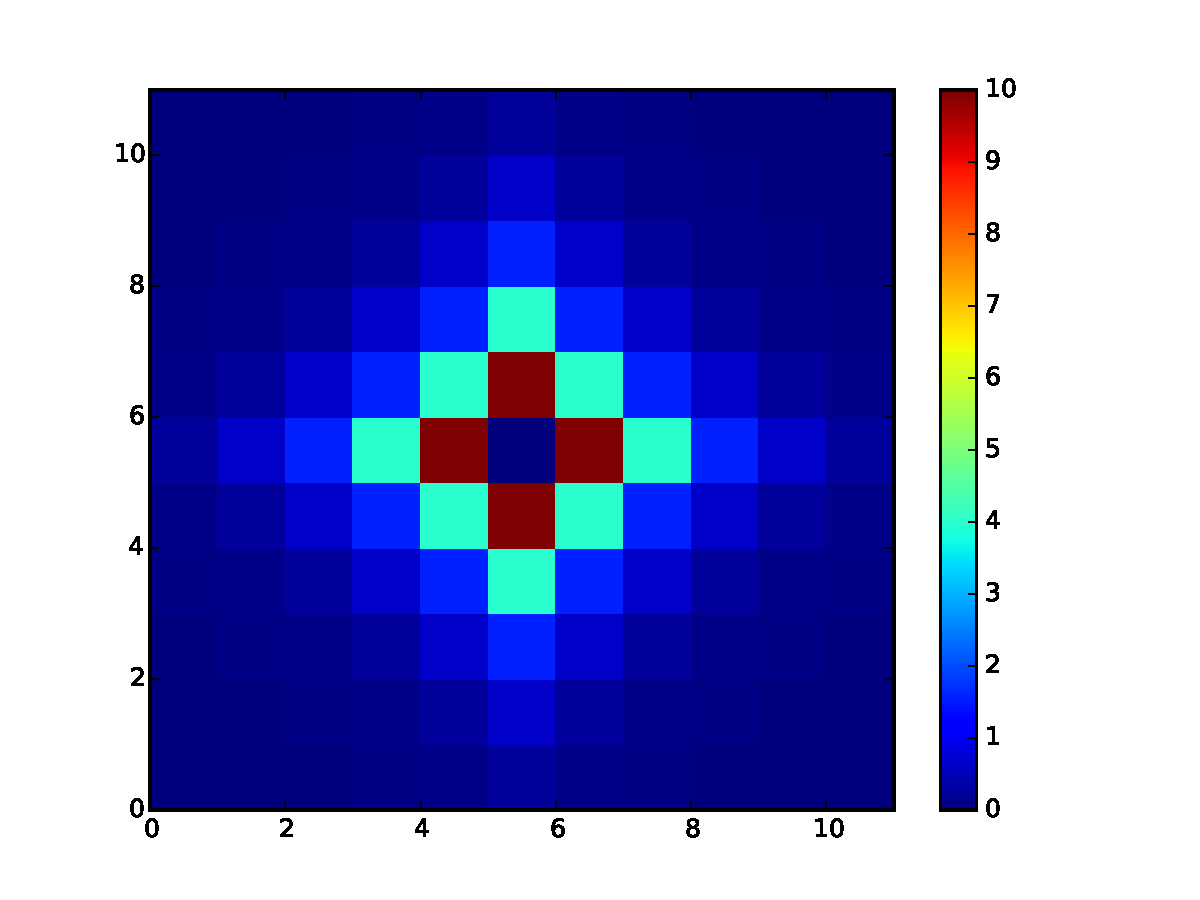
\includegraphics[width=\textwidth]{valueiteration_gamma0-5}
    \caption{$\gamma$ = 0.5}\label{fig:1b}
  \end{subfigure}
  \quad
  \begin{subfigure}[t]{.45\textwidth}
    \centering
    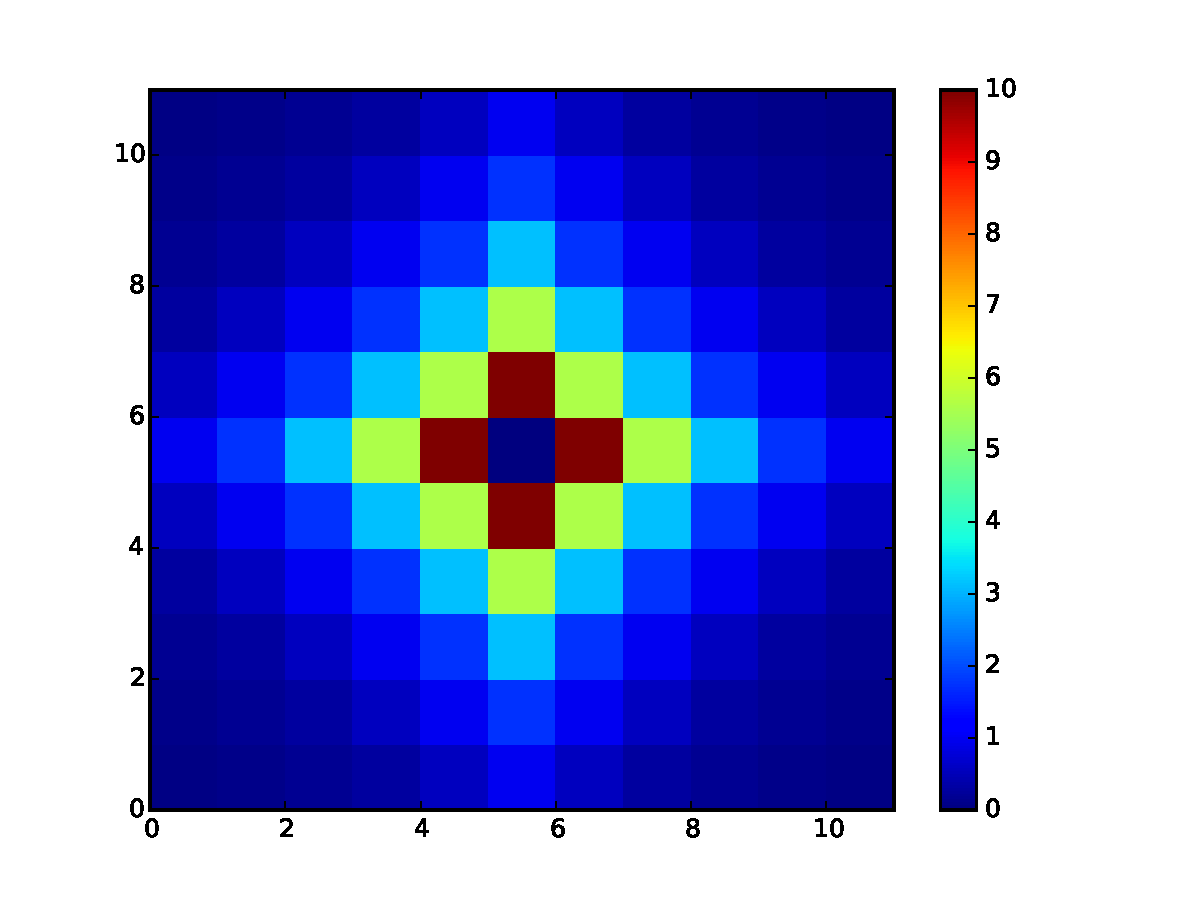
\includegraphics[width=\textwidth]{valueiteration_gamma0-7}
    \caption{$\gamma$ = 0.7}\label{fig:1b}
  \end{subfigure}
  \quad
  \begin{subfigure}[t]{.45\textwidth}
    \centering
    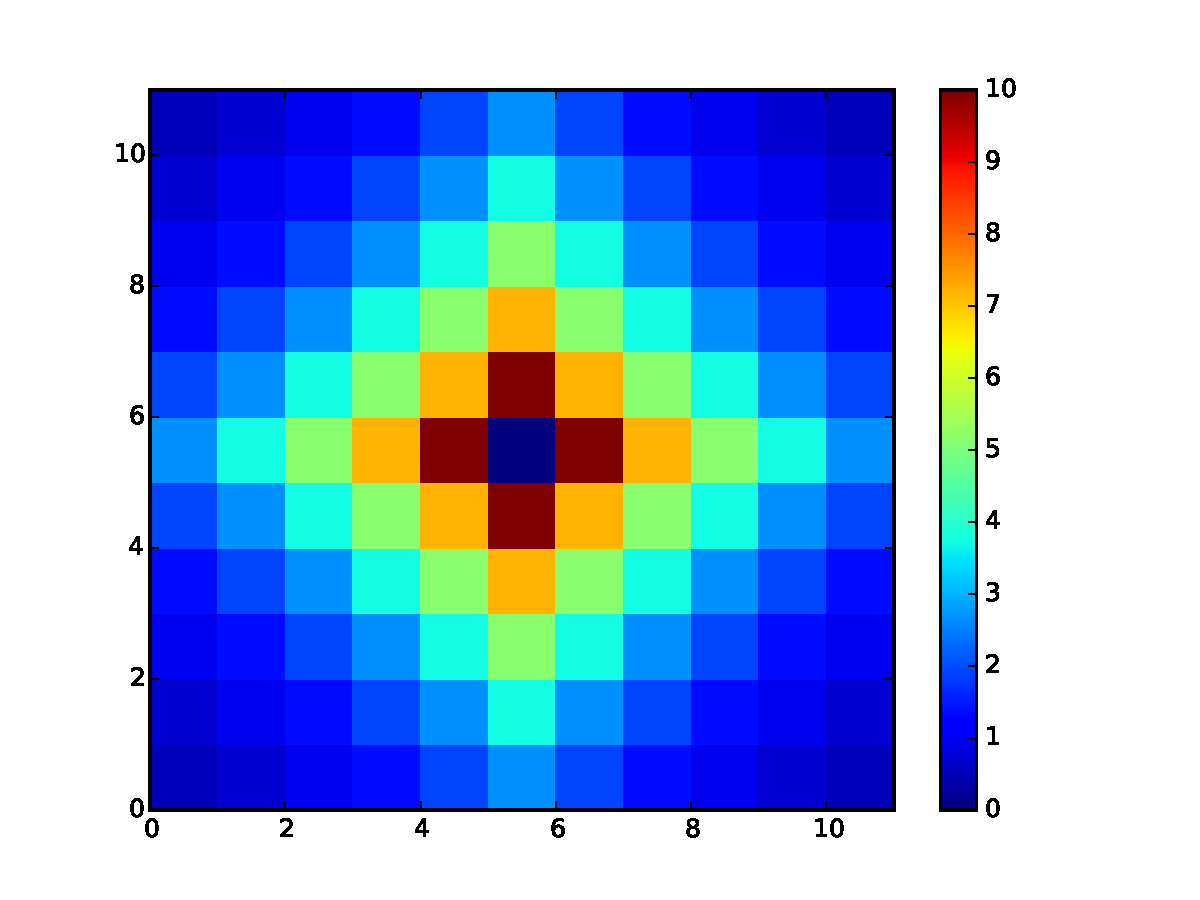
\includegraphics[width=\textwidth]{valueiteration_gamma0-9}
    \caption{$\gamma$ = 0.9}\label{fig:1b}
  \end{subfigure}
  \caption{Heatmaps of the final values for prey(5,5), illustrating the effect of the discount factor $\gamma$}\label{fig:1}
\end{figure}

\section{Question 5: Relative Position}
We implemented a relative position in our code, but due to time constraints we were not able to get it working with the functions above. We considered encoding the state space as the Manhattan Distance from the Predator to the Prey. This reduces the size of the state space from $(11 \times 11)*(11 \times 11) = 14.641$ to $10 \times 10 = 100$. 

We illustrate in figure~\ref{fig:state_diagram} how the state would change, given an action of the predator and the stochastic movement of the prey. Say the predator is at location 5,5 and the prey at 7,8 in the 11x11 grid. We would then encode the state as (2,3). If the predator then moves down, and the prey moved up, the new state would be (0,3). 

One thing that needs to be considered when using this state encoding is the toroidal grid. E.g. state (2,5) is followed by state (2,-5) when the predator moves left (and the prey stays).

\begin{figure}[h!]
	\centering
    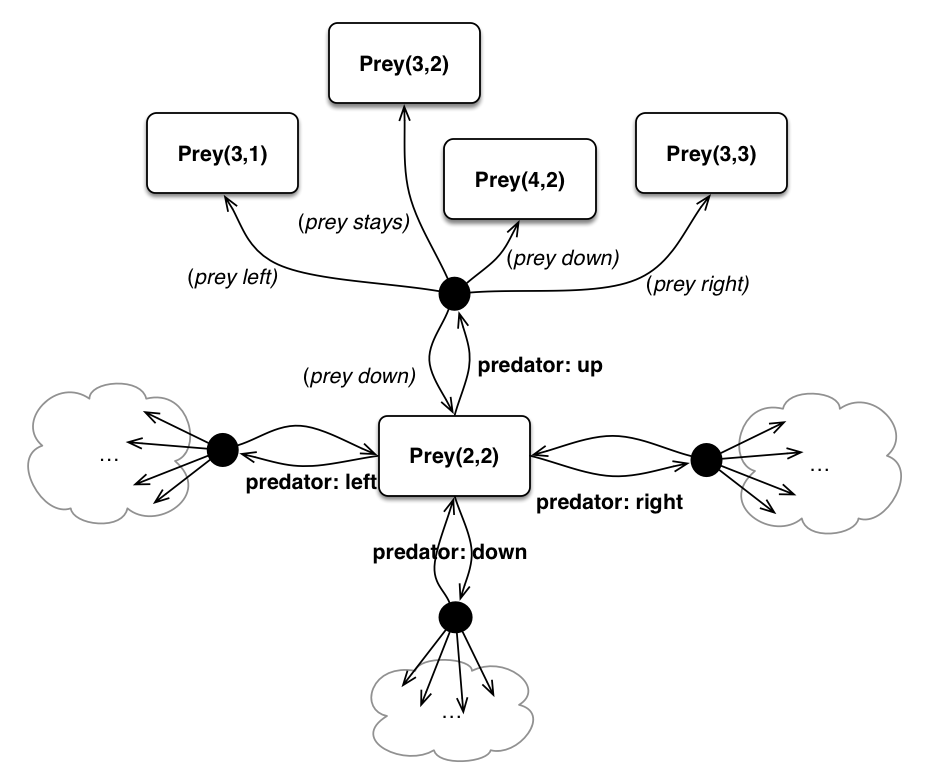
\includegraphics[width=0.75\textwidth]{state_diagram}
  \caption{State diagram for relative position}
   \label{fig:state_diagram}
\end{figure}
\section{Conclusion}
We have implemented the first 4 sub-assignments as explained in the assignment description. The relative position assignments was considered, but implementation was later removed in refactoring due to time constraints. We plan on implementing this before delving into Assignment 2.

The results presented in question 3 and 4 show that Value Iteration is faster than Policy Iteration (PI), both in iterations as well as in execution time. The higher computation time in PI can be attributed to the extra loop over the state space for the policy improvement step in PI. 
%\todo{anything else?}
\end{document}